\documentclass[a4paper]{article}
%\documentclass[8pt]{report}
%%%%%%%% CREATE DOCUMENT STRUCTURE %%%%%%%%
%% Language and font encodings
\usepackage[english]{babel}
\usepackage[utf8x]{inputenc}
\usepackage[T1]{fontenc}

%\usepackage{subfig}

%% Sets page size and margins
\usepackage[a4paper,top=3cm,bottom=2cm,left=2cm,right=2cm,marginparwidth=1.75cm]{geometry}

%% Useful packages
\usepackage{amsmath}
\usepackage{graphicx}
\usepackage[colorinlistoftodos]{todonotes}
\usepackage[colorlinks=true, allcolors=blue]{hyperref}
%\usepackage{caption}
\usepackage[justification=centering]{caption}
\usepackage{subcaption}
\usepackage{sectsty}
\usepackage{float}
\usepackage{titling} 
\usepackage{blindtext}
\usepackage[square,sort,comma,numbers]{natbib}
\usepackage[colorinlistoftodos]{todonotes}
\usepackage{xcolor}
\usepackage{fancyhdr}
\usepackage{lipsum}
\usepackage{amsfonts} 

%% definitions 
\definecolor{darkgreen}{rgb}{0.0, 0.4, 0.0}

%% Define your personal info here %%%%%%%%%%%%%%%%%%%%%%%
\newcommand\TPid{1}
\newcommand\TPname{Linear Algebra}
\newcommand\Firstname{Joao Filipe}
\newcommand\Familyname{Costa da Quinta}
\newcommand\Email{Joao.Costa@etu.unige.ch}

%%%%%%%%%%%%%%%%%%%%%%%%%%%%%%%%%%%%%%%%%%%%%%%%%%%%%%%

%%%%%%% Page header %%%%%%
\pagestyle{fancy}
\fancyhf{}
\rhead{TP \TPid: \TPname}
\lhead{\Firstname \Familyname}
\rfoot{Page \thepage}


%%%%%%%% DOCUMENT %%%%%%%%
\begin{document}

%%%% Title Page
\begin{titlepage}

\newcommand{\HRule}{\rule{\linewidth}{0.5mm}} 							% horizontal line and its thickness

\center 
 
% University
\textsc{\LARGE Université de Genève}\\[1cm]

% Document info
\textsc{\Large Data Science}\\[0.2cm]									% Course Code
\HRule \\[0.8cm]
{ \huge \bfseries TP \TPid : \TPname}\\[0.7cm]								% Assignment
\HRule \\[2cm]
\large
\emph{Author:} \Firstname \; \Familyname\\[0.5cm]		
\emph{E-mail:} {\color{blue}\Email}\\[7cm]		
% Author info
% Author info
{\large \today}\\[2cm]

\includegraphics[width=0.4\textwidth]{images/unige_csd.png}\\[1cm] 	% University logo
\vfill 
\end{titlepage}


% ============================================
% ----------------------------------
\newpage
\section*{1 - Matrix}
\subsection*{.1}
$$\begin{cases}a + b + c = 1\\ 4a + 2b + c = 9 \\ 9a + 3b + c =27\end{cases} \Leftrightarrow  \begin{cases} a=5\\b=-7\\c=3\end{cases}$$
\begin{itemize}
\item[(1)] We can start by writing the first equation: ${\color{red}\longrightarrow} c = 1 -a -b$
\item[(2)] insert step (1) in equation 2 and write it: ${\color{red}\longrightarrow} 4a +2b +1 -a -b = 9 \Leftrightarrow 3a + b = 8 \Leftrightarrow b = 8 - 3a$
\item[(3)] Rewrite $c = 1 -a -b$: ${\color{red}\longrightarrow} c = 1 -a -(8 - 3a) \Leftrightarrow c = -7 + 2a$
\item[(4)] Insert equations from (3) and (2) into equation 3:${\color{red}\longrightarrow} 9a + 3*(8 - 3a) + (-7 + 2a) = 27$
\item[(5)] Solve step (4): ${\color{red}\longrightarrow} 9a + 24 -9a -7 +2a = 27 \Leftrightarrow a = 5$
\item[(6)] Insert step (5) into step (2):${\color{red}\longrightarrow} b = 8 -3*5 \Leftrightarrow b = -7$
\item[(7)] Insert steps (5) and (6) into step (1): ${\color{red}\longrightarrow} c = 1 - 5 + 7 \Leftrightarrow c = 3$
\end{itemize}


\subsection*{.2}
$$\begin{cases}x + ay = 2\\ bx + 2y = 3\end{cases} \Leftrightarrow \begin{cases}x = 2 - ay\\ bx + 2y = 3\end{cases}$$
We can now insert the $1^{st}$ equation into the $2^{nd}$ equation as follows:\\
$b(2 - ay) + 2y = 3 \Leftrightarrow 2b - aby + 2y = 3 \Leftrightarrow 2b - y(ab -2) = 3 \Leftrightarrow y = (-1) * \left( \frac{3 - 2b}{(ab - 2)} \right) $\\
With given $a$ and $b$ values we can easily compute $y$, then we reinsert $y$ into the first equation to get $x$.
% ----------------------------------
\section*{2 - The importance of the mathematical concept behind a code}
\subsection*{.1}
\textbf{$def \ project\_on\_first(u, v)$} receives two column vectors as an argument, and it projects v onto u, the projected vector is usually called v', in the image bellow it is represented by $\vec{w_{1}}^{\,}$. Visually, it means that v' and u are collinear. This also means that: $\exists\ \alpha \in \mathbb{R}$ tq. $v'*\alpha = u$.
\begin{figure}[H]
\center
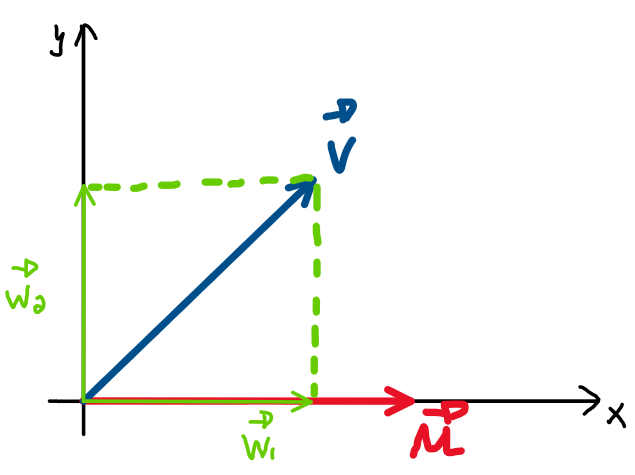
\includegraphics[width=0.3\textwidth]{images/projection.PNG}
\caption{Projection of $\vec{v}^{\,}$ onto $\vec{u}^{\,}$ = $\vec{w_{1}}^{\,}$}
\end{figure}
\subsection*{.2}
\textbf{zip()} function takes as argument two python lists of same size. It then merges one value from the first list, with another value from the second list (same index), creating a list of tuples. \\
Let's see an example:
\begin{center}
x = zip([1,2], [3,4]) -> x = [(1,3),(2,4)]
\end{center}
This means that the three last lines of code perform a simple dot operation between the two vectors given as argument to zip().
\begin{center}
It can be rewritten as: r = np.dot(u,v)
\end{center}
\subsection*{.3}
Step 1: find the vector $\vec{w_{2}}^{\,}$ orthogonal to $\vec{u}^{\,}$\\
If we look at Figure 1, we can see that $\vec{w_{1}}^{\,}$ is collinear to $\vec{u}^{\,}$, and that $\vec{w_{2}}^{\,}$ is orthogonal to $\vec{u}^{\,}$. Moreover, $\vec{v}^{\,}$ = $\vec{w_{1}}^{\,}$ + $\vec{w_{2}}^{\,}$, which means we can easily compute $\vec{w_{2}}^{\,}$ if we have already computed $\vec{w_{1}}^{\,}$. 
\begin{center}
$\vec{w_{2}}^{\,}$ = $\vec{v}^{\,}$ - $\vec{w_{1}}^{\,}$
\end{center}
Step 2: Make it so the orthogonal vector $\vec{w_{2}}^{\,}$ has the same norm as vector $\vec{u}^{\,}$\\
We must first compute $||\vec{u}^{\,}||$ as well as $||\vec{w_{2}}^{\,}||$.\\
By multiplying $\vec{w_{2}}^{\,}$ by a given real value $\alpha$ we can find a new vector $\vec{w_{2}'}^{\,}$ that is collinear to $\vec{w_{2}}^{\,}$, but of different norm.
\begin{center}
$\alpha$ = $||\vec{u}^{\,}||$ / $||\vec{w_{2}}^{\,}||$
\end{center}
\textbf{$def\ orthogonal\_norm\_on\_first(u, v)$} is the function inside $some\_script.py$ that does this computation.

% ----------------------------------
\section*{3 - Computing Eigenvalues, Eigenvectors, and Determinants}
\subsection*{.1}
$$ Det(A) = Det\left( \begin{matrix} 1 & 1 & 3 \\ 1 & 5 & 1 \\ 3 & 1 & 1 \end{matrix} \right)$$
$1 * Det \left( \begin{matrix} 5 & 1 \\ 1 & 1 \end{matrix} \right) - 1 * Det \left( \begin{matrix} 1 & 1 \\ 3 & 1 \end{matrix} \right) + 3 * Det \left( \begin{matrix} 1 & 5 \\ 3 & 1 \end{matrix} \right) = 1 * (5 - 1) -1 * (1 - 3) + 3 * (1 - 15) = 4 + 2 -42 = -36$\\
The computer returned the same value.\\
To compute eigenvalues and eigenvectors we have to compute the characteristic polynomial, P(A):\\
$$ P(A) = Det(A - I\lambda)= 0 <=> Det\left( \begin{matrix} (1 - \lambda) & 1 & 3 \\ 1 & (5 - \lambda) & 1 \\ 3 & 1 & (1 - \lambda) \end{matrix} \right) = 0$$

$(1 - \lambda) * Det \left( \begin{matrix} (5 - \lambda) & 1 \\ 1 & (1 - \lambda) \end{matrix} \right) - 1 * Det \left( \begin{matrix} 1 & 1 \\ 3 & (1 - \lambda) \end{matrix} \right) + 3 * Det \left( \begin{matrix} 1 & (5 - \lambda) \\ 3 & 1 \end{matrix} \right) $\\$= (1 - \lambda) * (4 - 6\lambda + \lambda^{2}) - 1 * (2 + \lambda) + 3 * (1 - 15 + 3\lambda) = -36 + 7\lambda^{2} - \lambda^{3} = -(\lambda + 2)(\lambda - 3)(\lambda - 6)$\\
This means our eigenvalues are: $\{-2, +3, +6\}$, now we just have to compute the respective eigenvectors. This is done in the following way:
$$(A - I\lambda) = \left(\begin{matrix} x \\ y \\ z \end{matrix}\right) = \left(\begin{matrix} 0 \\ 0 \\ 0 \end{matrix}\right), \lambda = \{-2, +3, +6\} $$
Once we solve it we get the respective eigenvectors:
$$\lambda = 6 \longrightarrow \left(\begin{matrix} 1 \\ 2 \\ 1 \end{matrix}\right), \lambda = 3 \longrightarrow \left(\begin{matrix} 1 \\ -1 \\ 1 \end{matrix}\right), \lambda = -2 \longrightarrow \left(\begin{matrix} -1 \\ 0 \\ 1 \end{matrix}\right)$$

\subsection*{.2}
\subsection*{.3}
\textbf{$tp\_1\_exercise\_3\_3.ipynb$} is the file with all the code for this exercise.

% ----------------------------------
\section*{4 - Computing Projection Onto a Line}
\subsection*{.1}
The distance is $~3.61$.\\
\textbf{$def\ compute\_distance\_line\_a()$} is the function inside $some\_script.py$ that does this computation.
\subsection*{.2}
We have a function $\alpha : 3x - 2y = -6$ that describes a line, and we have a point $A(5, 4)$. Let's see the steps required to compute the distance between $A$ and $f$, figure 2 is a sketch of what is explained in the item bellow:
\begin{itemize}
\item[(1)] We can rewrite it as $y = f(x) = \frac{-6 -3x}{-2}$
\item[(2)] Choose two values for x, and compute the respective images: $f(x_{1}) = y_{1}$ and $f(x_{2}) = y_{2}$
\item[(3)] Compute a vector $\vec{u}^{\,}$ that is collinear to our function $f$, $\vec{u}^{\,} = \begin{bmatrix} x_{2} - x_{1}\\y_{2} - y_{1} \end{bmatrix}$
\item[(4)] Compute $\vec{v}^{\,}$, vector between a point of the function $f$ and our point $A$, $\vec{v}^{\,} = \begin{bmatrix}  A_{x} - x_{1}\\ A_{y} - y_{1} \end{bmatrix}$
\item[(5)] Compute $\vec{w_{1}}^{\,}$ the projection of $\vec{v}^{\,}$ onto $\vec{u}^{\,}$, $\vec{w_{1}}^{\,}$ and $\vec{u}^{\,}$ are collinear
\item[(6)] Compute $\vec{w_{2}}^{\,}$ = $\vec{v}^{\,}$ - $\vec{w_{1}}^{\,}$, $\vec{w_{2}}^{\,}$ is orthogonal to $\vec{u}^{\,}$
\item[(7)] Compute $||\vec{w_{2}}^{\,}||$, which is the distance between the point $A$ and the line represented by the function $f$
\end{itemize}

\begin{figure}[H]
\center
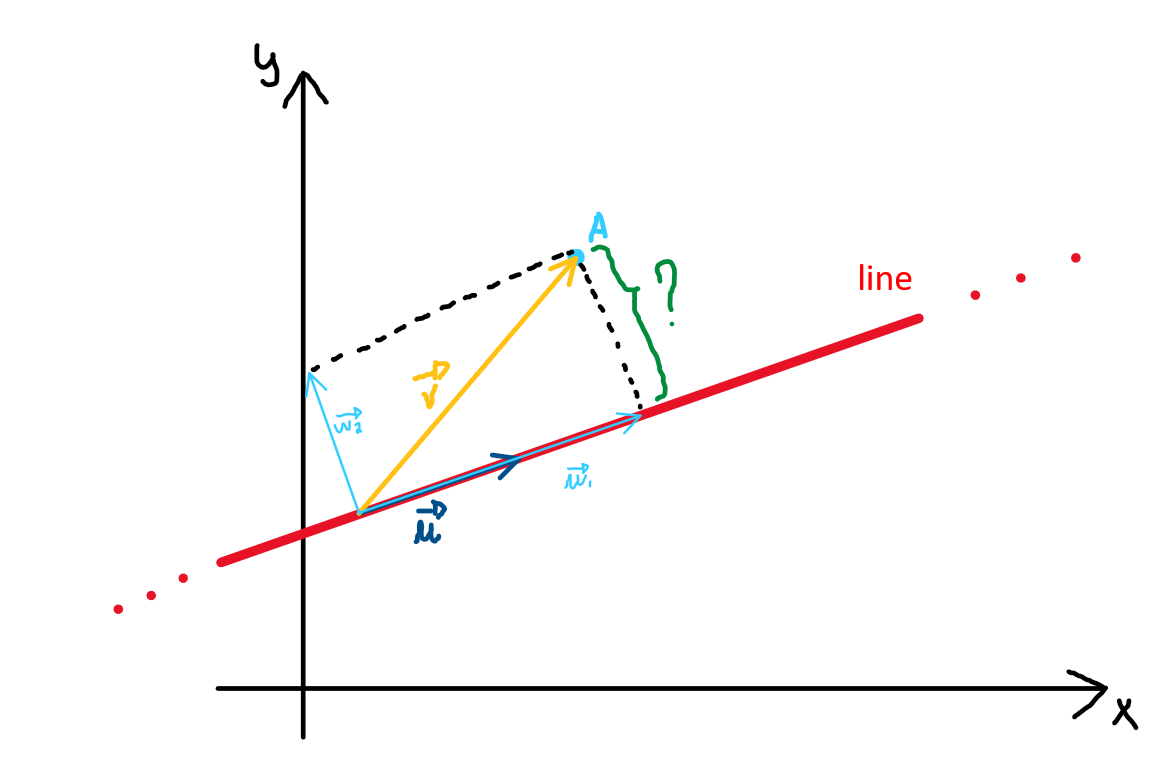
\includegraphics[width=0.7\textwidth]{images/projection_exo_4.PNG}
\caption{Distance between line and a point A}
\end{figure}



\end{document}
